\documentclass[11pt,a4paper]{article}

\usepackage[utf8]{inputenc}
\usepackage[T1]{fontenc}
\usepackage[french]{babel}
\usepackage[margin=2.5cm]{geometry}
\setlength{\parskip}{0.35cm}
\setlength{\parindent}{1em}
\usepackage{graphicx}
\usepackage{booktabs}
\usepackage{amsmath}
\usepackage{amssymb}
\usepackage{hyperref}
\usepackage{xcolor}
\usepackage{caption}
\captionsetup{justification=centering}
\usepackage{listings}
\usepackage{tikz}
\usepackage[most]{tcolorbox}
\usepackage{float}
\usetikzlibrary{arrows.meta,positioning}

\newtcolorbox{propobox}[1]{colback=gray!10, colframe=gray!50!black,
boxrule=0.5pt, arc=2pt, left=8pt, right=8pt, top=6pt, bottom=6pt,
title={#1}, fonttitle=\bfseries, coltitle=black, colbacktitle=gray!25}

\lstset{basicstyle=\ttfamily\small, breaklines=true, columns=fullflexible}

\definecolor{linkdark}{rgb}{0.35,0.05,0.05}
\definecolor{citedark}{rgb}{0.05,0.25,0.15}
\hypersetup{
    colorlinks=true,
    linkcolor=linkdark,
    citecolor=citedark,
    urlcolor=linkdark
}

\title{Un LLM dans l'algorithme A* sans forcément casser les garanties théoriques ?}
\author{ABDELOUHAB Yacine et JANIN Paul \\ M2 IASD App \\ Projet Modélisation de Problèmes}
\date{Juillet 2026}

\begin{document}
\maketitle

\vfill
\begin{abstract}
\begin{center}
\begin{minipage}{0.85\textwidth}
\setlength{\parindent}{2em}

A* recherche un chemin entre un état de départ et un état but dans un graphe d'états. Il garantit de trouver le chemin de coût minimal parmi tous les chemins possibles entre ces deux états. Pour cela, A* évalue chaque état par une fonction f, qui additionne le coût déjà payé pour atteindre l'état et une estimation du coût restant appelée heuristique. Trois points d'insertion se distinguent naturellement dans l'algorithme. On se demande alors s'il est possible d'y insérer un LLM sans casser la garantie d'optimalité, et si oui à quel prix. Deux de ces trois points peuvent être rendus théoriquement sûrs moyennant des protections précises. Le gain mesuré reste pourtant nul ou négligeable, même sur les niveaux faciles.

On casse ensuite volontairement ces garanties en reproduisant le
mécanisme du papier LLM-A*, où le LLM n'est plus protégé du tout. Le
gain en efficacité est net sur la recherche de chemin, mais nettement
plus incertain sur Taquin et Sokoban, où l'espace de dispositions
possibles est bien plus grand. Sur l'instance la plus difficile de
Taquin, cette liberté totale casse même l'optimalité et ralentit la
recherche au lieu de l'accélérer.
\end{minipage}
\end{center}
\end{abstract}
\vfill

\newpage
\begingroup
\setlength{\parskip}{0pt}
\tableofcontents
\endgroup
\newpage

% ============================================================
\section{Introduction}
% ============================================================

\subsection{Résumé de A*}

A* est un algorithme de recherche qui trouve le chemin le moins coûteux entre un état de départ et un état but, dans un ensemble d'états reliés entre eux par des actions possibles. Pour chaque état qu'il découvre, A* retient un coût $g$, qui est le prix déjà payé pour l'atteindre depuis le départ, et une estimation $h$ du coût qui reste à payer pour atteindre le but depuis cet état.

\smallskip
\noindent Cette estimation $h$ est appelée \textbf{l'heuristique}, et son rôle est de guider la recherche vers le but sans avoir à tout explorer. A* combine ces deux quantités en une valeur $f = g + h$ pour chaque état, et explore toujours en priorité l'état de plus petite valeur de $f$ parmi ceux qu'il connaît déjà mais n'a pas encore explorés.

\smallskip
\indent
Cette règle simple donne à A* sa \textbf{garantie d'optimalité}. Si l'heuristique ne surestime jamais le vrai coût restant, alors le premier état but que A* explore est nécessairement atteint par le chemin le moins coûteux possible. La figure~\ref{fig:astar-toy} illustre ce mécanisme sur un petit exemple.

\begin{figure}[H]
\centering
\begin{tikzpicture}[
    >={Stealth[length=2.5mm]},
    state/.style={circle, draw, minimum size=1cm},
    lbl/.style={font=\small, inner sep=1pt}
]
    \node[state] (E0) at (0,0) {$e_{\text{init}}$};
    \node[state] (E1) at (3,2.2) {$e_1$};
    \node[state] (E2) at (3,0) {$e_2$};
    \node[state] (E3) at (3,-2.2) {$e_3$};
    \node[state] (BUT) at (6.4,2.2) {but};

    \draw[->, thick] (E0) -- node[lbl, above] {2} (E1);
    \draw[->, thick] (E0) -- node[lbl, above] {2} (E2);
    \draw[->, thick] (E0) -- node[lbl, below] {1} (E3);
    \draw[->, thick] (E1) -- node[lbl, above] {1} (BUT);
    \draw[->, thick] (E2) -- node[lbl, below right] {3} (BUT);

    \node[lbl, below=3pt of E0] {$g=0,\ h=3$};
    \node[lbl, above=3pt of E1] {$g=2,\ h=2$};
    \node[lbl, below=3pt of E2] {$g=2,\ h=2$};
    \node[lbl, below=3pt of E3] {$g=1,\ h=4$};
    \node[lbl, above=3pt of BUT] {$h=0$};
\end{tikzpicture}
\caption{Exemple jouet, en deux temps.}
\label{fig:astar-toy}
\end{figure}

\textbf{Premier temps}

Depuis $e_{\text{init}}$, A* génère trois voisins.
\begin{itemize}
    \item $e_1$ : coût 2, reste estimé 2, $f(e_1) = 4$.
    \item $e_2$ : coût 2, reste estimé 2, $f(e_2) = 4$, égalité avec $e_1$.
    \item $e_3$ : coût 1, reste estimé 4, $f(e_3) = 5$.
\end{itemize}
$e_1$ et $e_2$ sont à égalité, avec le $f$ le plus petit. A* choisit arbitrairement l'un des deux, par exemple $e_1$, et laisse $e_2$ disponible.

\textbf{Deuxième temps}

A* explore $e_1$ et découvre \emph{but}, à coût 1
de plus, $f(\text{but}) = g(e_1)+1+0 = 3$. C'est désormais la plus petite valeur parmi les états à explorer ($e_2$ à $f=4$, $e_3$ à $f=5$), donc A* explore \emph{but} et s'arrête.

\subsection{Identification des points d'entrée pour un LLM}

L'algorithme A* prend, à chaque étape, plusieurs petites décisions, et
certaines d'entre elles pourraient en principe être confiées à un grand
modèle de langage plutôt qu'à une règle fixe. Trois de ces décisions se
distinguent naturellement.

\begin{itemize}
    \item Le choix de l'état à explorer en premier.
    \item Le calcul de l'estimation $h$ elle-même, qui pourrait être produite par un LLM à partir d'une description de l'état, plutôt que calculée par une formule fixe.
    \item La décision d'écarter définitivement un état jugé sans issue, avant même de l'explorer.
\end{itemize}

Ces trois décisions n'ont pas le même effet sur la garantie d'optimalité de A*, et c'est précisément ce que ce rapport étudie en détail dans la section~\ref{sec:points}.

\subsection{Le mécanisme du papier LLM-A*}

Le papier \textbf{LLM-A*} \cite{meng2024llmastar} propose une approche différente, qui n'agit sur aucune des trois décisions ci-dessus. Il fait générer par un LLM une liste d'états appelés \textbf{waypoints}. Il s'agit de points de passage intermédiaires plausibles entre le départ et le but. On modifie ensuite directement la fonction d'évaluation de A* en y ajoutant un troisième terme
\[
f(s) = g(s) + h(s) + \mathrm{cout\_vers\_cible}(\text{cible actuelle}, s)
\]
où $\mathrm{cout\_vers\_cible}$ mesure la distance restante entre l'état $s$ et le prochain waypoint à atteindre, et où le waypoint courant change au fil de la recherche à mesure que les précédents sont atteints. 

\smallskip
\noindent
Ce troisième terme guide donc activement la recherche vers le prochain waypoint plutôt que directement vers le but. Il est cependant fourni par un LLM, sans aucune propriété garantie, ni admissibilité ni consistance, et rien dans la méthode du papier ne borne l'écart entre la solution trouvée et l'optimum réel.

\subsection{Question de recherche}

Ce projet part d'une idée inverse. Peut-on insérer un LLM à des points précis d'un algorithme A* générique, choisis parce qu'on peut analyser leur impact sur l'optimalité, et parfois le neutraliser ? Et si oui pour certains points mais pas pour d'autres, quel est le prix réel de cette sûreté, en appels API et en gain mesuré ?

Nous répondons à cette question sur trois jeux, la recherche de chemin sur grille, le taquin, et Sokoban. Ces trois jeux diffèrent par le nombre d'actions possibles à chaque état, par la fréquence à laquelle un même état est atteignable par plusieurs chemins différents, et par la présence ou non de véritables impasses.

\subsection{Plan du rapport}

La section~\ref{sec:points} détaille les trois points d'insertion identifiés, avec pour chacun une analyse théorique de sa garantie. La section~\ref{sec:waypoints} reproduit et étend le mécanisme du papier LLM A* sur nos trois jeux. La section~\ref{sec:experimentation} présente les résultats de nos expérimentations, et y répond directement.

% ============================================================
\section{Un algorithme A* générique et trois points d'insertion}
\label{sec:points}
% ============================================================

L'algorithme A* du projet (\texttt{Algorithmes/A\_etoile/a\_etoile.py}) est écrit pour rester générique, et permet de faire intervenir un LLM aux trois endroits identifiés dans l'introduction.

\begin{enumerate}
    \item \textbf{Ordonner les nœuds à explorer} (\texttt{departager\_llm}), où le LLM choisit, parmi des états \emph{à f strictement égal}, lequel explorer en premier.
    \item \textbf{Calculer l'heuristique d'un nœud} (\texttt{heuristique\_llm\_lot}), où le LLM remplace entièrement $h(\text{état})$.
    \item \textbf{Élaguer les états} (\texttt{elaguer\_llm}), où le LLM décide si un état candidat doit être définitivement écarté des ouverts.
\end{enumerate}

Ces trois points n'ont pas le même statut vis-à-vis de la garantie d'optimalité, et c'est précisément ce qui en fait un objet d'étude intéressant.

\subsection{Quel état choisir pour l'exploration ? (point d'insertion 1)}

A* doit décider, à chaque étape, lequel des états déjà connus mais pas encore explorés il va traiter ensuite\footnote{Dans notre code, cet ensemble correspond à la liste \texttt{ouverts}, et les états déjà traités, dans \texttt{fermes}, ne sont plus reconsidérés.}. Un LLM pourrait sembler bien placé pour cette décision, à partir d'une description de chaque candidat. Le problème est que rien ne garantit la façon dont il va trancher parmi cette liste. L'optimalité de A* n'est garantie que si l'état retenu est toujours celui de plus petite valeur de $f$.

Or, en pratique, plusieurs états partagent souvent cette plus petite valeur de $f$, et pas un seul. Ceci est visible sur l'exemple de la figure~\ref{fig:astar-toy}, mais aussi dans les jeux considérés ici. Si on force donc le LLM à ne recevoir en entrée que cet ensemble d'états à $f$ minimal, et à trancher uniquement parmi eux, l'optimalité reste garantie, par construction.

C'est exactement ce que fait \texttt{departager\_llm}. On modélise l'ensemble des états à explorer par un tas (\texttt{heapq}), on dépile ceux qui partagent la même valeur de $f$, et on les propose au LLM, qui choisit lequel explorer en premier. Il ne choisit donc que parmi les états ayant le score le plus petit. Les états non choisis sont remis dans le tas. En pratique, ce gain reste toutefois modeste, et même nul sur les niveaux les plus difficiles, un point développé en section~\ref{sec:experimentation}.

\subsection{Peut on remplacer l'heuristique par un LLM ? (point d'insertion 2)}
\label{sec:point2}

A* a besoin d'une estimation du coût restant pour chaque état, c'est l'heuristique $h$. Un LLM pourrait sembler bien placé pour trouver cette estimation, à partir d'une description de l'état, plutôt que de la calculer avec une formule fixe. C'est exactement ce que fait \texttt{heuristique\_llm\_lot}, qui remplace entièrement $h(\text{état})$. On présente au LLM l'ensemble des états voisins nouvellement découverts, au moment de l'expansion d'un nœud, et on lui demande d'estimer le coût restant pour chacun.

Contrairement au point 1, ce choix change directement quelle valeur de $f$ est la plus petite. La garantie d'optimalité n'est donc plus automatique. Elle dépend de propriétés que le LLM n'a aucune raison de respecter spontanément.

\begin{propobox}{Deux propriétés indépendantes}
Soit $h^*(\text{état})$ le vrai coût minimal restant depuis un état jusqu'à un but.

\medskip
Une heuristique $h$ est \textbf{admissible} si, pour tout état, $h(\text{état}) \le h^*(\text{état})$, c'est à dire si elle ne surestime jamais.

\medskip
Elle est \textbf{consistante}, une propriété plus forte, si pour tout état et tout voisin accessible en un pas de coût $c(\text{état}, \text{voisin})$, $h(\text{état}) \le c(\text{état}, \text{voisin}) + h(\text{voisin})$.

\medskip
La consistance implique l'admissibilité, mais l'inverse est faux.
\end{propobox}

Cette distinction est cruciale pour notre code parce que notre \texttt{a\_etoile()} ne rouvre jamais un état une fois placé dans \texttt{fermes} (\texttt{if etat\_suivant in fermes: continue}), une simplification standard qui n'est correcte que sous l'hypothèse de \textbf{consistance}. Avec une heuristique seulement admissible mais pas consistante, un état peut être fermé avec un $g$ non optimal, et un chemin moins cher découvert plus tard est alors purement ignoré. La consistance, et elle seule, garantit qu'un état fermé a toujours son coût optimal.

\subsubsection*{Contre-exemple}

La figure~\ref{fig:contre-exemple} montre le graphe construit pour ce
test, avec l'heuristique $h$ indiquée sous chaque état.

\begin{figure}[H]
\centering
\begin{tikzpicture}[
    >={Stealth[length=2.5mm]},
    state/.style={circle, draw, minimum size=0.9cm},
    lbl/.style={font=\small, inner sep=1pt}
]
    \node[state] (E0) at (0,0) {$e_{\text{init}}$};
    \node[state] (E1) at (2,1.4) {$e_1$};
    \node[state] (E2) at (4,0) {$e_2$};
    \node[state] (E3) at (6.2,0) {$e_3$};
    \node[state] (BUT) at (8.4,0) {but};

    \draw[->, thick] (E0) -- node[lbl, above left] {1} (E1);
    \draw[->, thick] (E0) -- node[lbl, below] {3} (E2);
    \draw[->, thick] (E1) -- node[lbl, above right] {1} (E2);
    \draw[->, thick] (E2) -- node[lbl, above] {1} (E3);
    \draw[->, thick] (E3) -- node[lbl, above] {1} (BUT);

    \node[lbl, below=3pt of E0] {$h=4$};
    \node[lbl, above=3pt of E1] {$h=3$};
    \node[lbl, below=3pt of E2] {$h=0$};
    \node[lbl, below=3pt of E3] {$h=1$};
    \node[lbl, below=3pt of BUT] {$h=0$};
\end{tikzpicture}
\caption{Illustration de l'importance de la consistance}
\label{fig:contre-exemple}
\end{figure}

Le vrai optimum est $e_{\text{init}} \to e_1 \to e_2 \to e_3 \to
\text{but}$, de coût 4. Vérifions l'admissibilité, état par état, avec
$h^*(\text{état})$ le vrai coût restant jusqu'à \emph{but}.
\begin{itemize}
    \item $h(e_{\text{init}}) = 4 \le h^*(e_{\text{init}}) = 4$.
    \item $h(e_1) = 3 \le h^*(e_1) = 3$.
    \item $h(e_2) = 0 \le h^*(e_2) = 2$.
    \item $h(e_3) = 1 \le h^*(e_3) = 1$.
    \item $h(\text{but}) = 0 \le h^*(\text{but}) = 0$.
\end{itemize}
Cette heuristique est donc admissible partout. Elle n'est cependant pas consistante. Prenons l'arête $e_1 \to e_2$. La consistance exigerait $h(e_1) \le c(e_1,e_2) + h(e_2)$, soit $3 \le 1+0=1$, ce qui est faux. Suivons maintenant, pas à pas, ce que fait notre \texttt{a\_etoile()} sur
ce graphe.

\begin{itemize}
    \item \textbf{Premier temps}, depuis $e_{\text{init}}$, $f(e_1)=1+3=4$
    et $f(e_2)=3+0=3$. A* explore $e_2$ en premier ($f$ plus petit), et le
    ferme avec $g(e_2)=3$. On explore donc plus jamais $e_2$ !
    
    \item \textbf{Deuxième temps}, A* explore $e_1$ et le ferme avec
    $g(e_1)=1$. Il redécouvre $e_2$ par un chemin moins cher ($g=2$ au
    lieu de 3), mais $e_2$ est déjà fermé, donc l'amélioration est
    ignorée (\texttt{if etat\_suivant in fermes: continue}).
    \item \textbf{Troisième temps}, A* continue avec le $g(e_2)=3$
    erroné, explore $e_3$ puis \emph{but}, et s'arrête sur un coût de 5,
    au lieu du vrai optimum de 4.
\end{itemize}

Une heuristique LLM seulement admissible reste donc exposée à un second risque, plus sournois, à savoir que rien ne garantit sa consistance d'un état à son voisin.

\subsubsection*{Deux parades testées simultanément}

Notons $h_{\text{llm}}$ l'heuristique renvoyée par le LLM, et
$h_{\text{classique}}$ l'heuristique classique du jeu, celle que
\texttt{a\_etoile()} utiliserait par défaut sans LLM. Chacune des deux parades ci-dessous protège une seule des deux propriétés.

\medskip
\noindent
Le \textbf{$\min(h_{\text{llm}}, h_{\text{classique}})$} protège l'admissibilité par construction. L'heuristique classique $h_{\text{classique}}$ est déjà admissible, donc
\[
h_{\text{classique}}(\text{état}) \le h^*(\text{état}) \quad \text{pour tout état.}
\]
Comme le minimum des deux est toujours inférieur ou égal à $h_{\text{classique}}$, on obtient directement
\[
\min(h_{\text{llm}}, h_{\text{classique}})(\text{état}) \le h^*(\text{état})
\]
pour tout état, quelle que soit la valeur renvoyée par le LLM. Ce mécanisme ne protège cependant pas la consistance.

\medskip
\noindent
La consistance demande :
\[
\text{pour chaque état, et chacun de ses voisins,} \quad h(\text{voisin}) \ge h(\text{état}) - \text{coût}(\text{état}, \text{voisin}).
\]
Le \textbf{pathmax} impose cette inégalité, mais seulement pour un seul
voisin à la fois, celui par lequel A* vient justement d'arriver, le
parent. À chaque pas parent vers voisin,
\[
h(\text{voisin}) = \max\big(h_{\text{llm}}(\text{voisin}),\ h(\text{parent}) - \text{coût}(\text{parent},\text{voisin})\big).
\]
Comme $h(\text{parent})$ est lui-même construit par la même règle depuis son propre parent, cette propriété se propage par récurrence à tout le chemin exploré depuis le départ. Le $\max()$ ne peut cependant jamais réduire une valeur. Pathmax ne corrige donc jamais une surestimation déjà présente dans $h_{\text{llm}}$.

Imposer une vraie consistance partout garantirait aussi l'admissibilité. Cela demanderait de connaître $h$ pour tous les
voisins d'un état, y compris ceux pas encore découverts par la recherche. Une recherche incrémentale ne peut pas anticiper ce calcul. La seule heuristique à la fois consistante et exacte serait $h^*$ lui-même, ce qui reviendrait à résoudre le problème avant de le chercher. Pathmax se limite donc à la relation parent-voisin, la seule information disponible sans coût supplémentaire, jamais à tous les couples état-voisin. Ce n'est donc jamais une vraie consistance globale. Le minimum, de son côté, protège seulement l'admissibilité.

\smallskip
\indent
Puisque la consistance impliquerait l'admissibilité, pathmax ne la garantit pas non plus. Aucune des deux parades ne suffit donc seule. Nos expérimentations activent donc toujours les deux ensemble par défaut, pour que les coûts mesurés restent fiables.

\subsubsection*{Version par lot}

On garde uniquement la version par lot, \texttt{heuristique\_llm\_lot},
pour toute la suite de ce rapport. Elle note tous les voisins nouveaux
d'un même nœud en un seul appel API, au lieu d'un appel par état. Sans
ça, le nombre d'appels API exploserait sur les niveaux réalistes.

\subsection{Peut on laisser un LLM écarter des états ? (point d'insertion 3)}
\label{sec:point3}

Contrairement aux points 1 et 2, \texttt{elaguer\_llm} n'a aucune protection possible. Dans \texttt{a\_etoile()}, \texttt{elaguer\_llm} est appelé au moment où un nouvel état voisin est découvert, avant même qu'il entre dans les ouverts. On lui soumet cet état, sans aucune garantie que son jugement soit correct. 

\medskip
\noindent
Si le LLM répond à tort que l'état est impossible, il est perdu pour toujours. Contrairement à une heuristique, qui influence
seulement l'ordre d'exploration, une mauvaise décision ici peut
supprimer la seule solution existante. A* ne la retrouvera jamais.

\subsubsection*{Vérification empirique sur quelques exemples}

On teste d'abord ce jugement sur des cas classiques, déjà bien
identifiés, comme :

\begin{itemize}
    \item[A.] Un coin mort certain, avec deux murs perpendiculaires et
    pas de cible. Il est bien impossible.
    \item[B.] Une caisse déjà sur sa cible. Il n'est pas impossible.
    \item[C.] Un bloc $2\times2$ de 4 caisses en pleine salle ouverte, un
    \textbf{freeze deadlock} où chaque caisse bloque les 3 autres sans
    qu'aucun mur ne soit nécessaire. Il est impossible, mais la règle
    classique ne le couvre pas, puisqu'aucun mur ne se trouve à
    proximité.
    \item[D.] Une caisse seule en pleine salle. Il n'est pas impossible.
\end{itemize}

Nous testons ces quatre états avec Claude Sonnet, selon deux variantes de prompt. Le \textbf{jugement libre} laisse le LLM juger librement. Le \textbf{raisonnement guidé} lui impose de vérifier explicitement chacune des 4 directions de poussée, pour chaque caisse.

\begin{table}[H]
\centering
\begin{tabular}{@{}lcccc@{}}
\toprule
Variante & A (coin) & B (cible) & C (freeze) & D (normal) \\
\midrule
Jugement libre & \textcolor{red}{Faux (raté)} & Correct & \textcolor{red}{Faux (raté)} & Correct \\
Raisonnement guidé & Correct & Correct & \textcolor{red}{Faux (raté)} & Correct \\
\bottomrule
\end{tabular}
\caption{Le jugement libre rate même le coin, le cas le plus évident. Le
raisonnement guidé corrige ce cas. Il rate cependant encore le
\emph{freeze deadlock}.}
\label{tab:elaguer-batterie}
\end{table}

Nous avons aussi testé et écarté une explication alternative, à savoir que le format de description de l'état changerait le résultat. Une grille détaillée avec des coordonnées explicites donne exactement le même résultat qu'une grille seule et minimale. Le raté n'est donc pas un problème de présentation du prompt, mais un vrai manque de vérification systématique de la mécanique de poussée.

Même sur ces cas classiques, pourtant simples, le LLM échoue déjà. C'est pourquoi la détection des cas classiques est placée clairement avant tout appel au LLM. Pour le problème du Sokoban, on repère ainsi une fois pour toutes ces cas simples et on laisse le LLM gérer les autres cas d'impossibilité.

L'élagage n'est testé que sur Sokoban, parmi nos trois jeux.
Recherche de chemin et Taquin n'ont pas de vrai cul-de-sac. Tout état atteint y reste résoluble. Tester l'élagage dessus ne voudrait rien dire.

Au vu de ces résultats, élaguer avec un LLM va sûrement être compliqué,
voire inefficace, surtout pour Sokoban, précisément le jeu où élaguer
serait le plus utile, sur un espace d'états qui peut croître de façon
exponentielle.


% ============================================================
\section{Reproduction du mécanisme du papier LLM-A*}
\label{sec:waypoints}
% ============================================================

Le papier LLM-A* laisse un LLM proposer librement des points de passage (waypoints), sans aucune garantie théorique, comme rappelé en section~\ref{sec:point2}. Pour comparer notre
approche à celle du papier original, nous avons reproduit et étendu ce mécanisme sur nos trois jeux. On veut savoir si, malgré la perte de la garantie d'optimalité, on gagne en efficacité en ne bridant pas le LLM comme le font les points d'insertion 1 et 2.

\subsection{Définitions d'un pathway pour chacun des jeux}

Un sous-objectif n'a de sens, pour Taquin ou pour Sokoban, qu'en tant qu'état complet. Nous généralisons donc le mécanisme du papier en \textbf{dispositions}, qui prennent une forme différente pour chacun de nos trois jeux.

\smallskip
\noindent
Pour Recherche de chemin, une disposition est directement une coordonnée $(x,y)$, comme le waypoint du papier original.

\smallskip
\noindent
Pour Taquin, une disposition est une permutation complète du plateau, puisqu'un sous-objectif partiel n'y a aucun sens.

\smallskip
\noindent
Pour Sokoban, une disposition est un ensemble complet de positions de caisses, optionnellement augmenté de la position du joueur.

\subsection{Un coût en appels API très différent}

Ce mécanisme demande un seul appel au LLM par instance, fait une fois avant même de démarrer la recherche, pour obtenir la liste complète des dispositions. La recherche se déroule ensuite entièrement de façon classique, sans plus jamais consulter le LLM. C'est une différence de plusieurs ordres de grandeur avec les points d'insertion 1 et 2, qui consomment jusqu'à 150 appels par instance. Cet appel unique reste cependant sans aucune garantie, contrairement aux points 1 et 2, ce qui en fait un compromis inverse, peu coûteux mais risqué, plutôt que sûr mais coûteux.

% ============================================================
\section{Expérimentation}
\label{sec:experimentation}
% ============================================================

\subsection{Définitions des heuristiques}

Chaque jeu garde sa propre heuristique classique, admissible car
construite comme un relâchement du vrai problème, une version plus
simple qui ignore une vraie contrainte et ne peut donc que sous-estimer
le coût restant. Pour Recherche de chemin, c'est la distance de
Manhattan vers le but, qui ignore les murs. Pour Taquin, c'est la somme
des distances de Manhattan de chaque pièce vers sa position finale, qui
ignore qu'un coup ne déplace qu'une seule pièce à la fois. Pour Sokoban,
c'est la somme des distances de Manhattan de la meilleure affectation
caisse vers cible, calculée avec l'\textbf{algorithme hongrois}
(\texttt{scipy.optimize.linear\_sum\_assignment}), qui ignore les murs
et le fait qu'on ne pousse qu'une seule caisse à la fois.

\subsection{Protocole}

Le pipeline officiel (\texttt{Resultat/lancer\_experimentation.py})
comprend 11 tâches indépendantes, une par instance, chacune comparant
une \textbf{baseline} classique aux points d'insertion 1 et 2, ainsi
qu'au point 3 pour Sokoban.

Sokoban est coupé en deux corpus distincts, microban et l'original de
1988. L'original est bien trop compliqué pour une recherche classique.
Son espace d'états explose avant même de trouver une solution
(table~\ref{tab:sweep}). Microban reste abordable, tout en gardant les
mêmes vraies mécaniques du jeu.

Les points d'insertion 1 et 2 consultent le LLM à chaque décision,
jusqu'à 150 fois par instance. Nous utilisons DeepSeek
(\texttt{deepseek-v4-pro}) pour ce pipeline systématique. Claude aurait
demandé le même nombre d'appels, à un coût bien plus élevé. Pour les
waypoints, un seul appel suffit par instance. Nous testons donc les
deux fournisseurs, Claude (\texttt{claude-sonnet-5}) et DeepSeek
(\texttt{deepseek-v4-pro}).

Nous construisons nous-mêmes chaque instance à la main.
\begin{itemize}
    \item Recherche de chemin, dans \texttt{Jeux/Recherche\_de\_chemin/exemples/}.
    \item Taquin, dans \texttt{Jeux/Taquin/exemples/}.
    \item Sokoban, dans \texttt{Jeux/Sokoban/exemples/}, pour microban et l'original.
\end{itemize}

\begin{itemize}
    \item Le \textbf{plafond d'états} arrête la recherche, sans solution, si
    elle explore trop d'états, pour ne jamais attendre indéfiniment sur un
    espace qui explose. Il est de 100\,000 pour les instances standard et
    de 250\,000 pour Sokoban original.
    \item Le \textbf{budget d'appels API} est de 150 par variante. Une fois ce
    budget épuisé, chaque hook retombe sur son comportement classique
    pour le reste de la recherche, ce qui évite tout blocage et tout coût
    illimité.
    \item Les instances couvrent plusieurs niveaux pour chaque jeu, avec
    une ou plusieurs cartes différentes par niveau (table~\ref{tab:sweep}).
\end{itemize}

\begin{table}[H]
\centering
\small
\begin{tabular}{@{}lcccc@{}}
\toprule
Jeu & niveau1 & niveau2 & niveau3 & niveau4 \\
\midrule
Recherche de chemin & 30--33 & 82--110 & 147--343 & 82--158 \\
Taquin & 4--17 & 34--83 & 18--68 & 12\,061--14\,606 \\
Sokoban (microban) & 1088--1088 & 1761--1761 & 13\,428--13\,428 & \textbf{56\,240--56\,240} \\
Sokoban (original, 1988) & \textbf{$\ge$200\,000, échec classique} & -- & -- & -- \\
\bottomrule
\end{tabular}
\caption{Nombre d'états explorés par A* classique, sans LLM,
minimum--maximum sur les cartes testées par niveau. Sokoban microban n'a qu'une carte par niveau. Taquin niveau4 est exclu, trop coûteux.}
\label{tab:sweep}
\end{table}

\subsection{Résultats pour Recherche de chemin}

\begin{table}[H]
\centering
\small
\resizebox{\textwidth}{!}{%
\begin{tabular}{@{}llccl@{}}
\toprule
Instance & Variante & Coût & Visites & Appels API \\
\midrule
niveau1\_facile & A* & 10 & 33 & 0 \\
niveau1\_facile & point 1 (\texttt{departager\_llm}) & 10 & 31 & 31 \\
niveau1\_facile & point 2 (\texttt{heuristique\_llm\_lot}) & 10 & 33 & 33 \\
\midrule
niveau1\_facile & LLM-A* & 10 & 14 (Claude, DeepSeek) & 1 \\
\midrule
niveau2\_moyen & A* & 21 & 110 & 0 \\
niveau2\_moyen & point 1 (\texttt{departager\_llm}) & 21 & 109 & 109 \\
niveau2\_moyen & point 2 (\texttt{heuristique\_llm\_lot}) & 21 & 110 & 106 \\
\midrule
niveau2\_moyen & LLM-A* & 21 & 30 (Claude, DeepSeek) & 1 \\
\midrule
niveau3\_difficile & A* & 42 & 171 & 0 \\
niveau3\_difficile & point 1 (\texttt{departager\_llm}) & 42 & 171 & 150 (budget épuisé) \\
niveau3\_difficile & point 2 (\texttt{heuristique\_llm\_lot}) & 42 & 171 & 150 (budget épuisé) \\
\midrule
niveau3\_difficile & LLM-A* & 42 & 81 (Claude), 67 (DeepSeek) & 1 \\
\bottomrule
\end{tabular}%
}
\caption{Recherche de chemin, tous les mécanismes comparés. Points 1 et
2 avec DeepSeek. LLM-A* avec Claude et DeepSeek.}
\label{tab:pathfinding-tout}
\end{table}

\begin{figure}[H]
\centering
\begin{minipage}{0.48\textwidth}
\centering
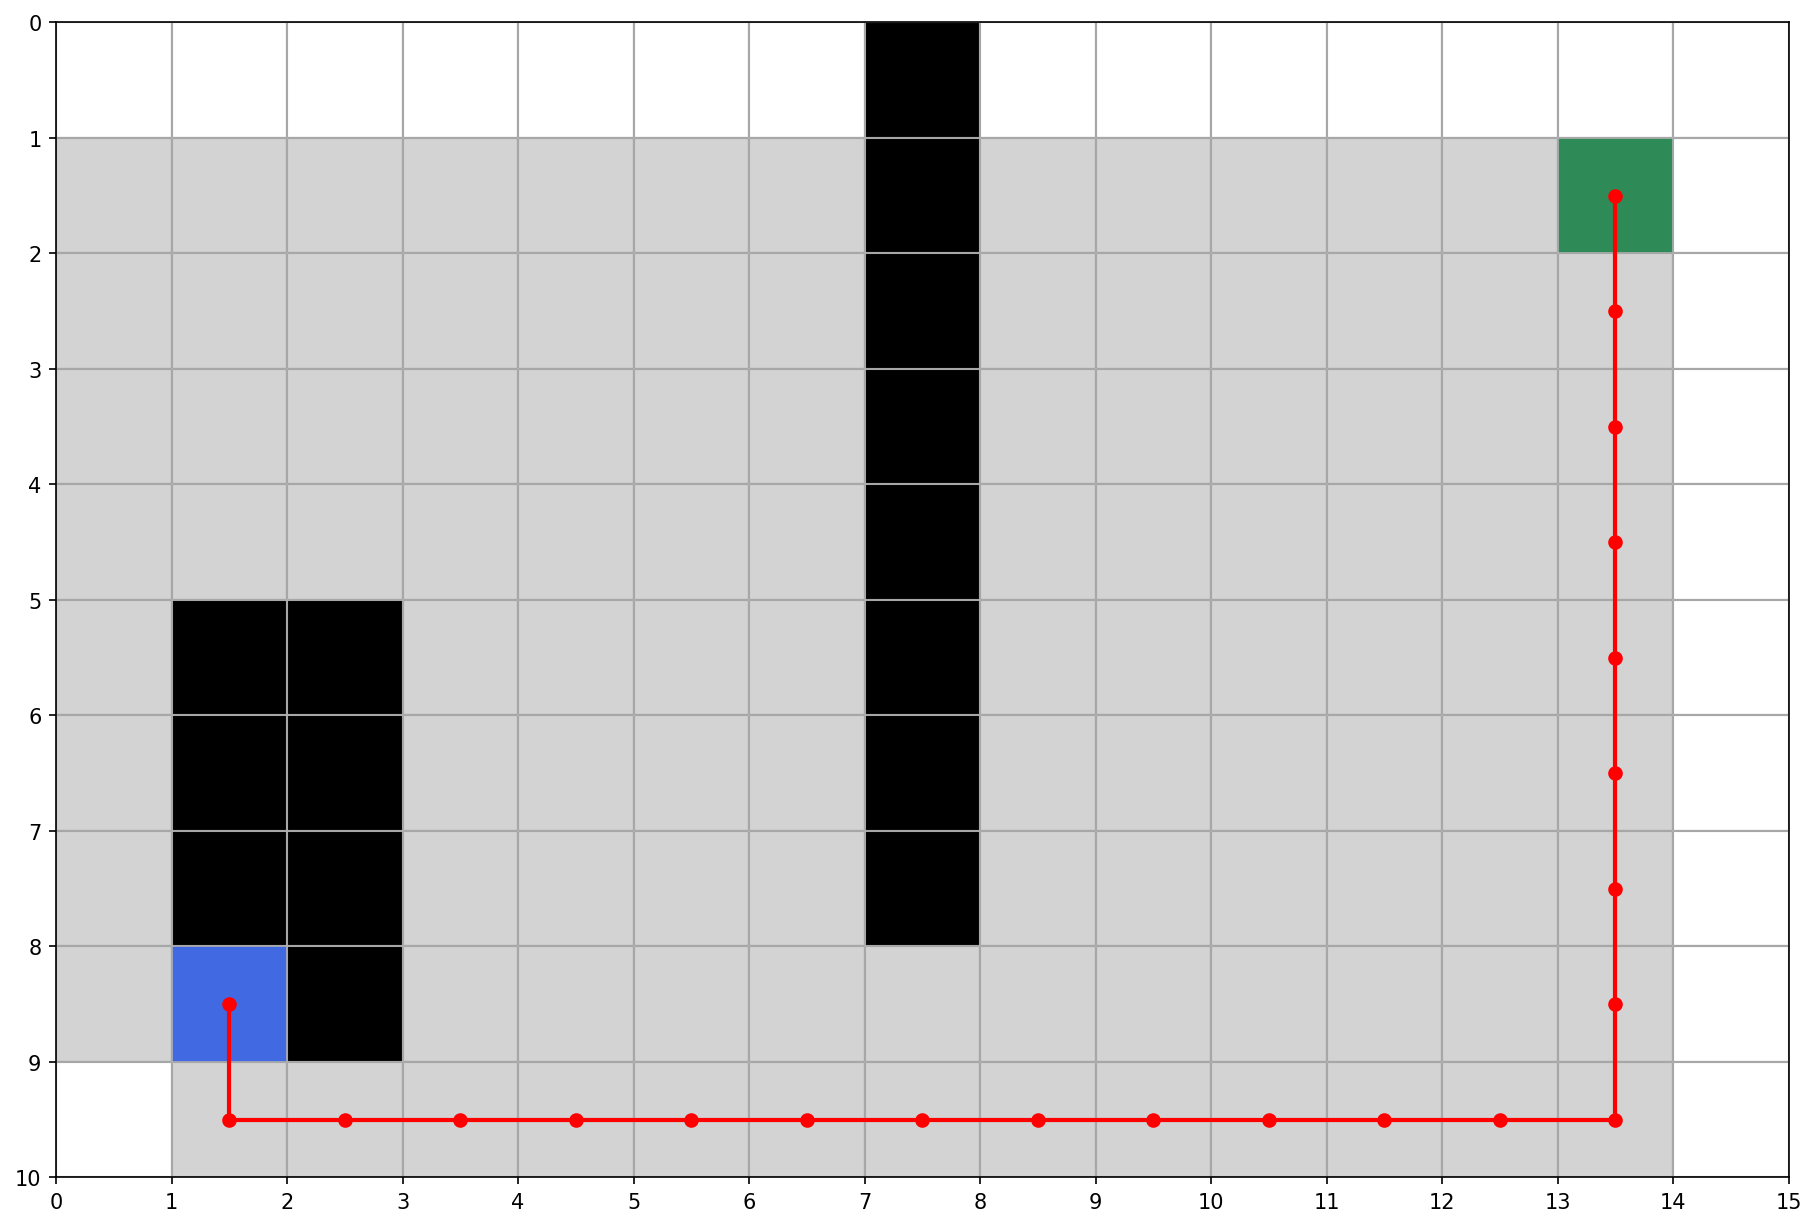
\includegraphics[width=\textwidth]{../Resultat/Recherche_de_chemin/Experimentation/visu_niveau2_moyen_baseline_etoile.png}
\end{minipage}
\hfill
\begin{minipage}{0.48\textwidth}
\centering
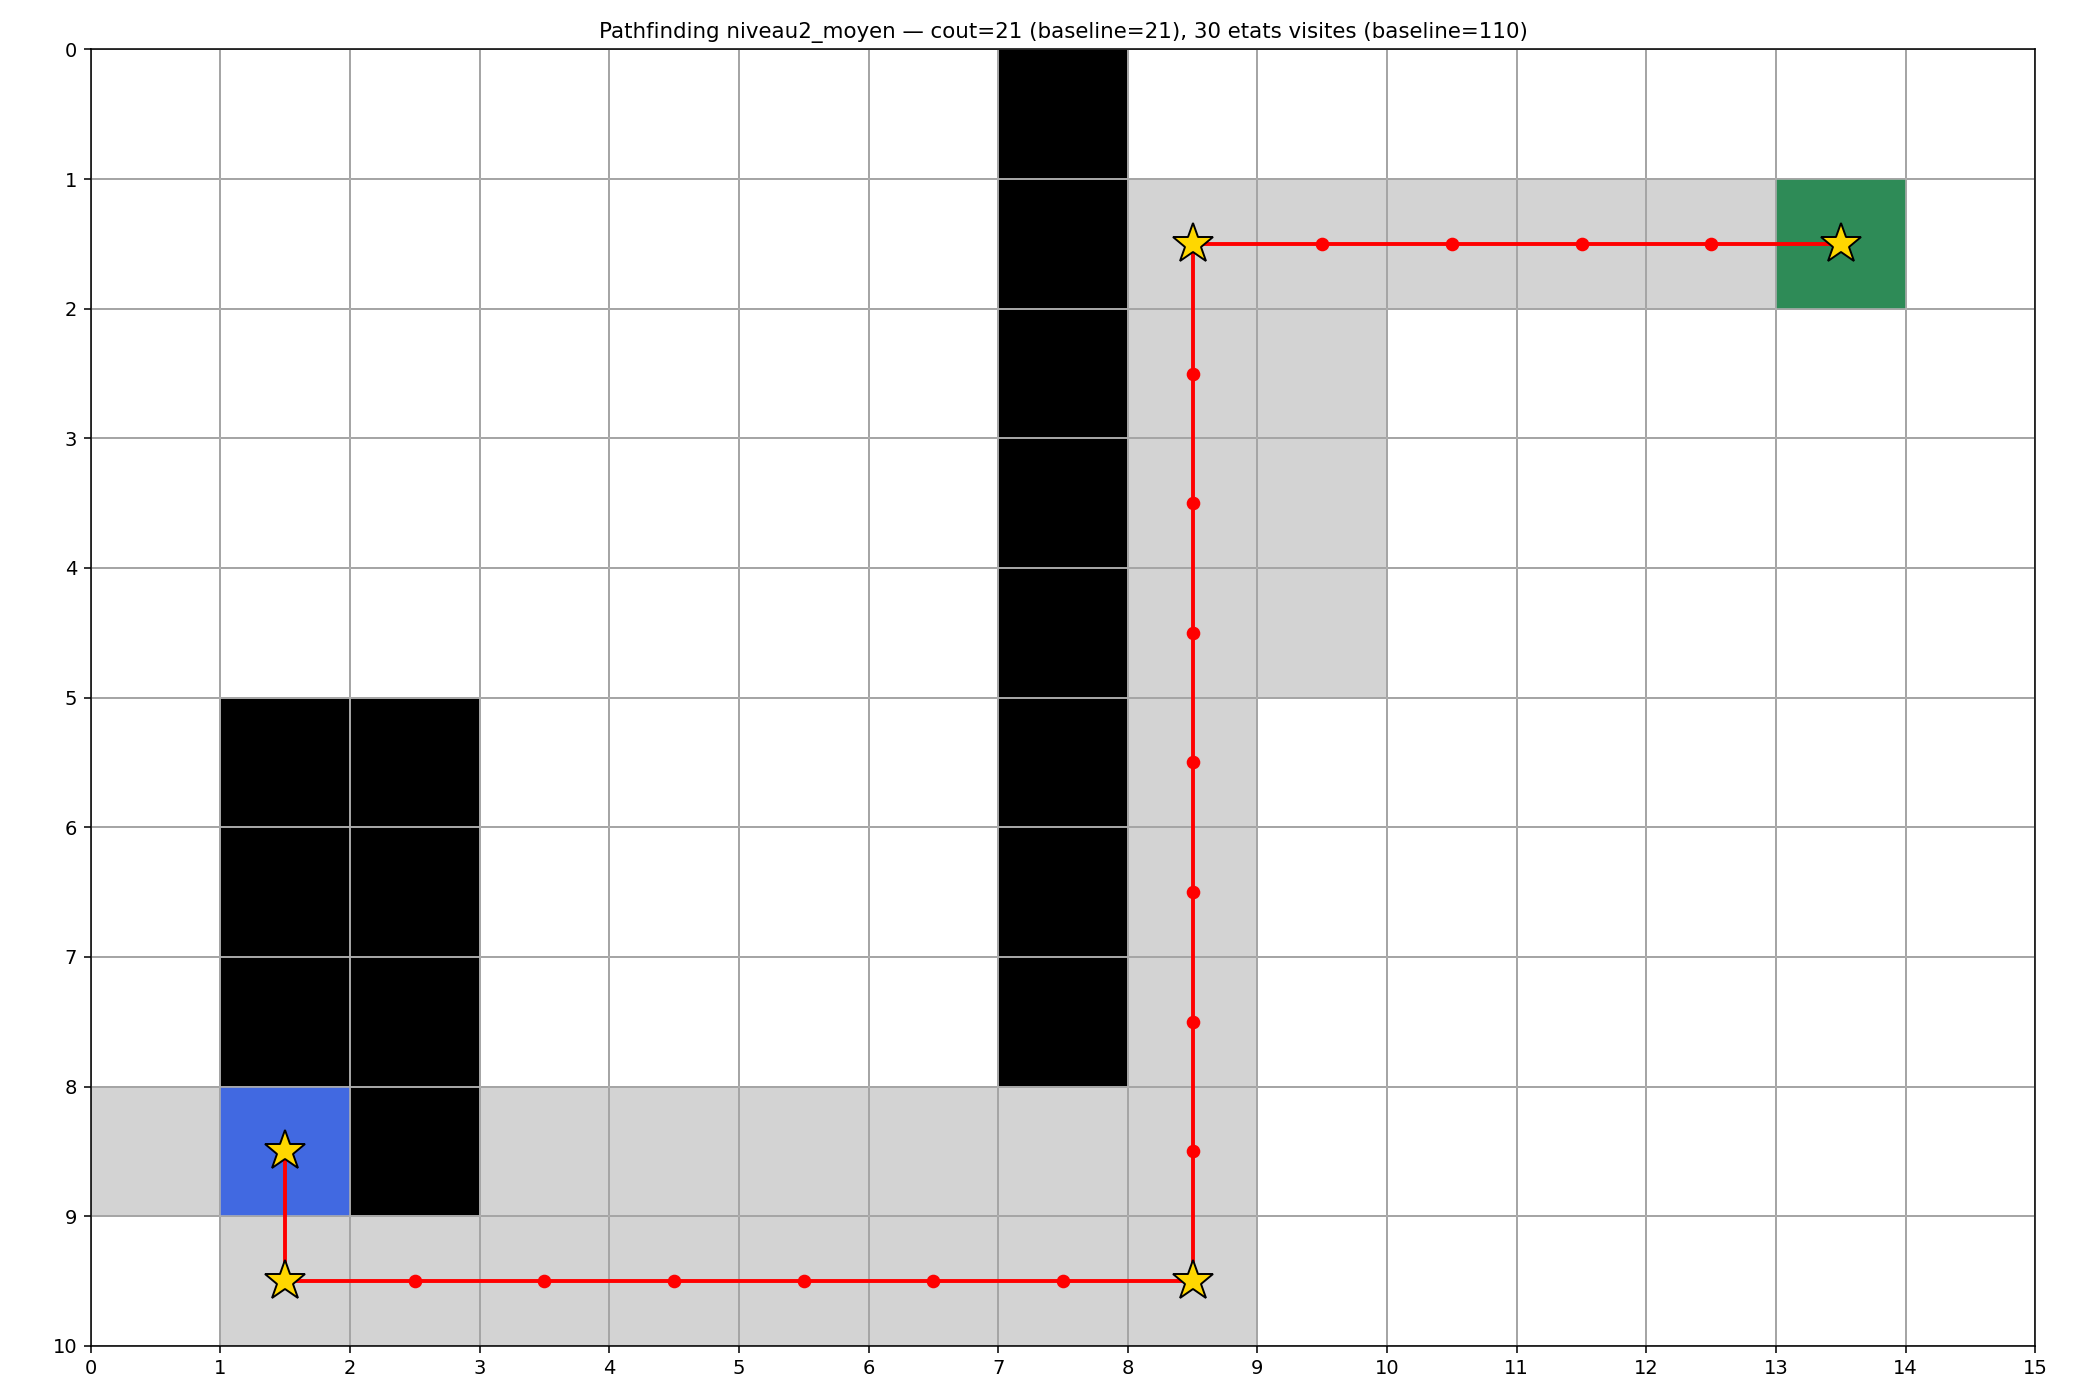
\includegraphics[width=\textwidth]{../Resultat/Recherche_de_chemin/Experimentation/visu_niveau2_moyen_waypoints_etoile.png}
\end{minipage}
\caption{Recherche de chemin niveau2\_moyen. À gauche, A* (110 états
visités). À droite, LLM-A* (30 états visités), à coût identique, avec
de points de passage intermédiaires.}
\end{figure}

\begin{figure}[H]
\centering
\begin{minipage}{0.48\textwidth}
\centering
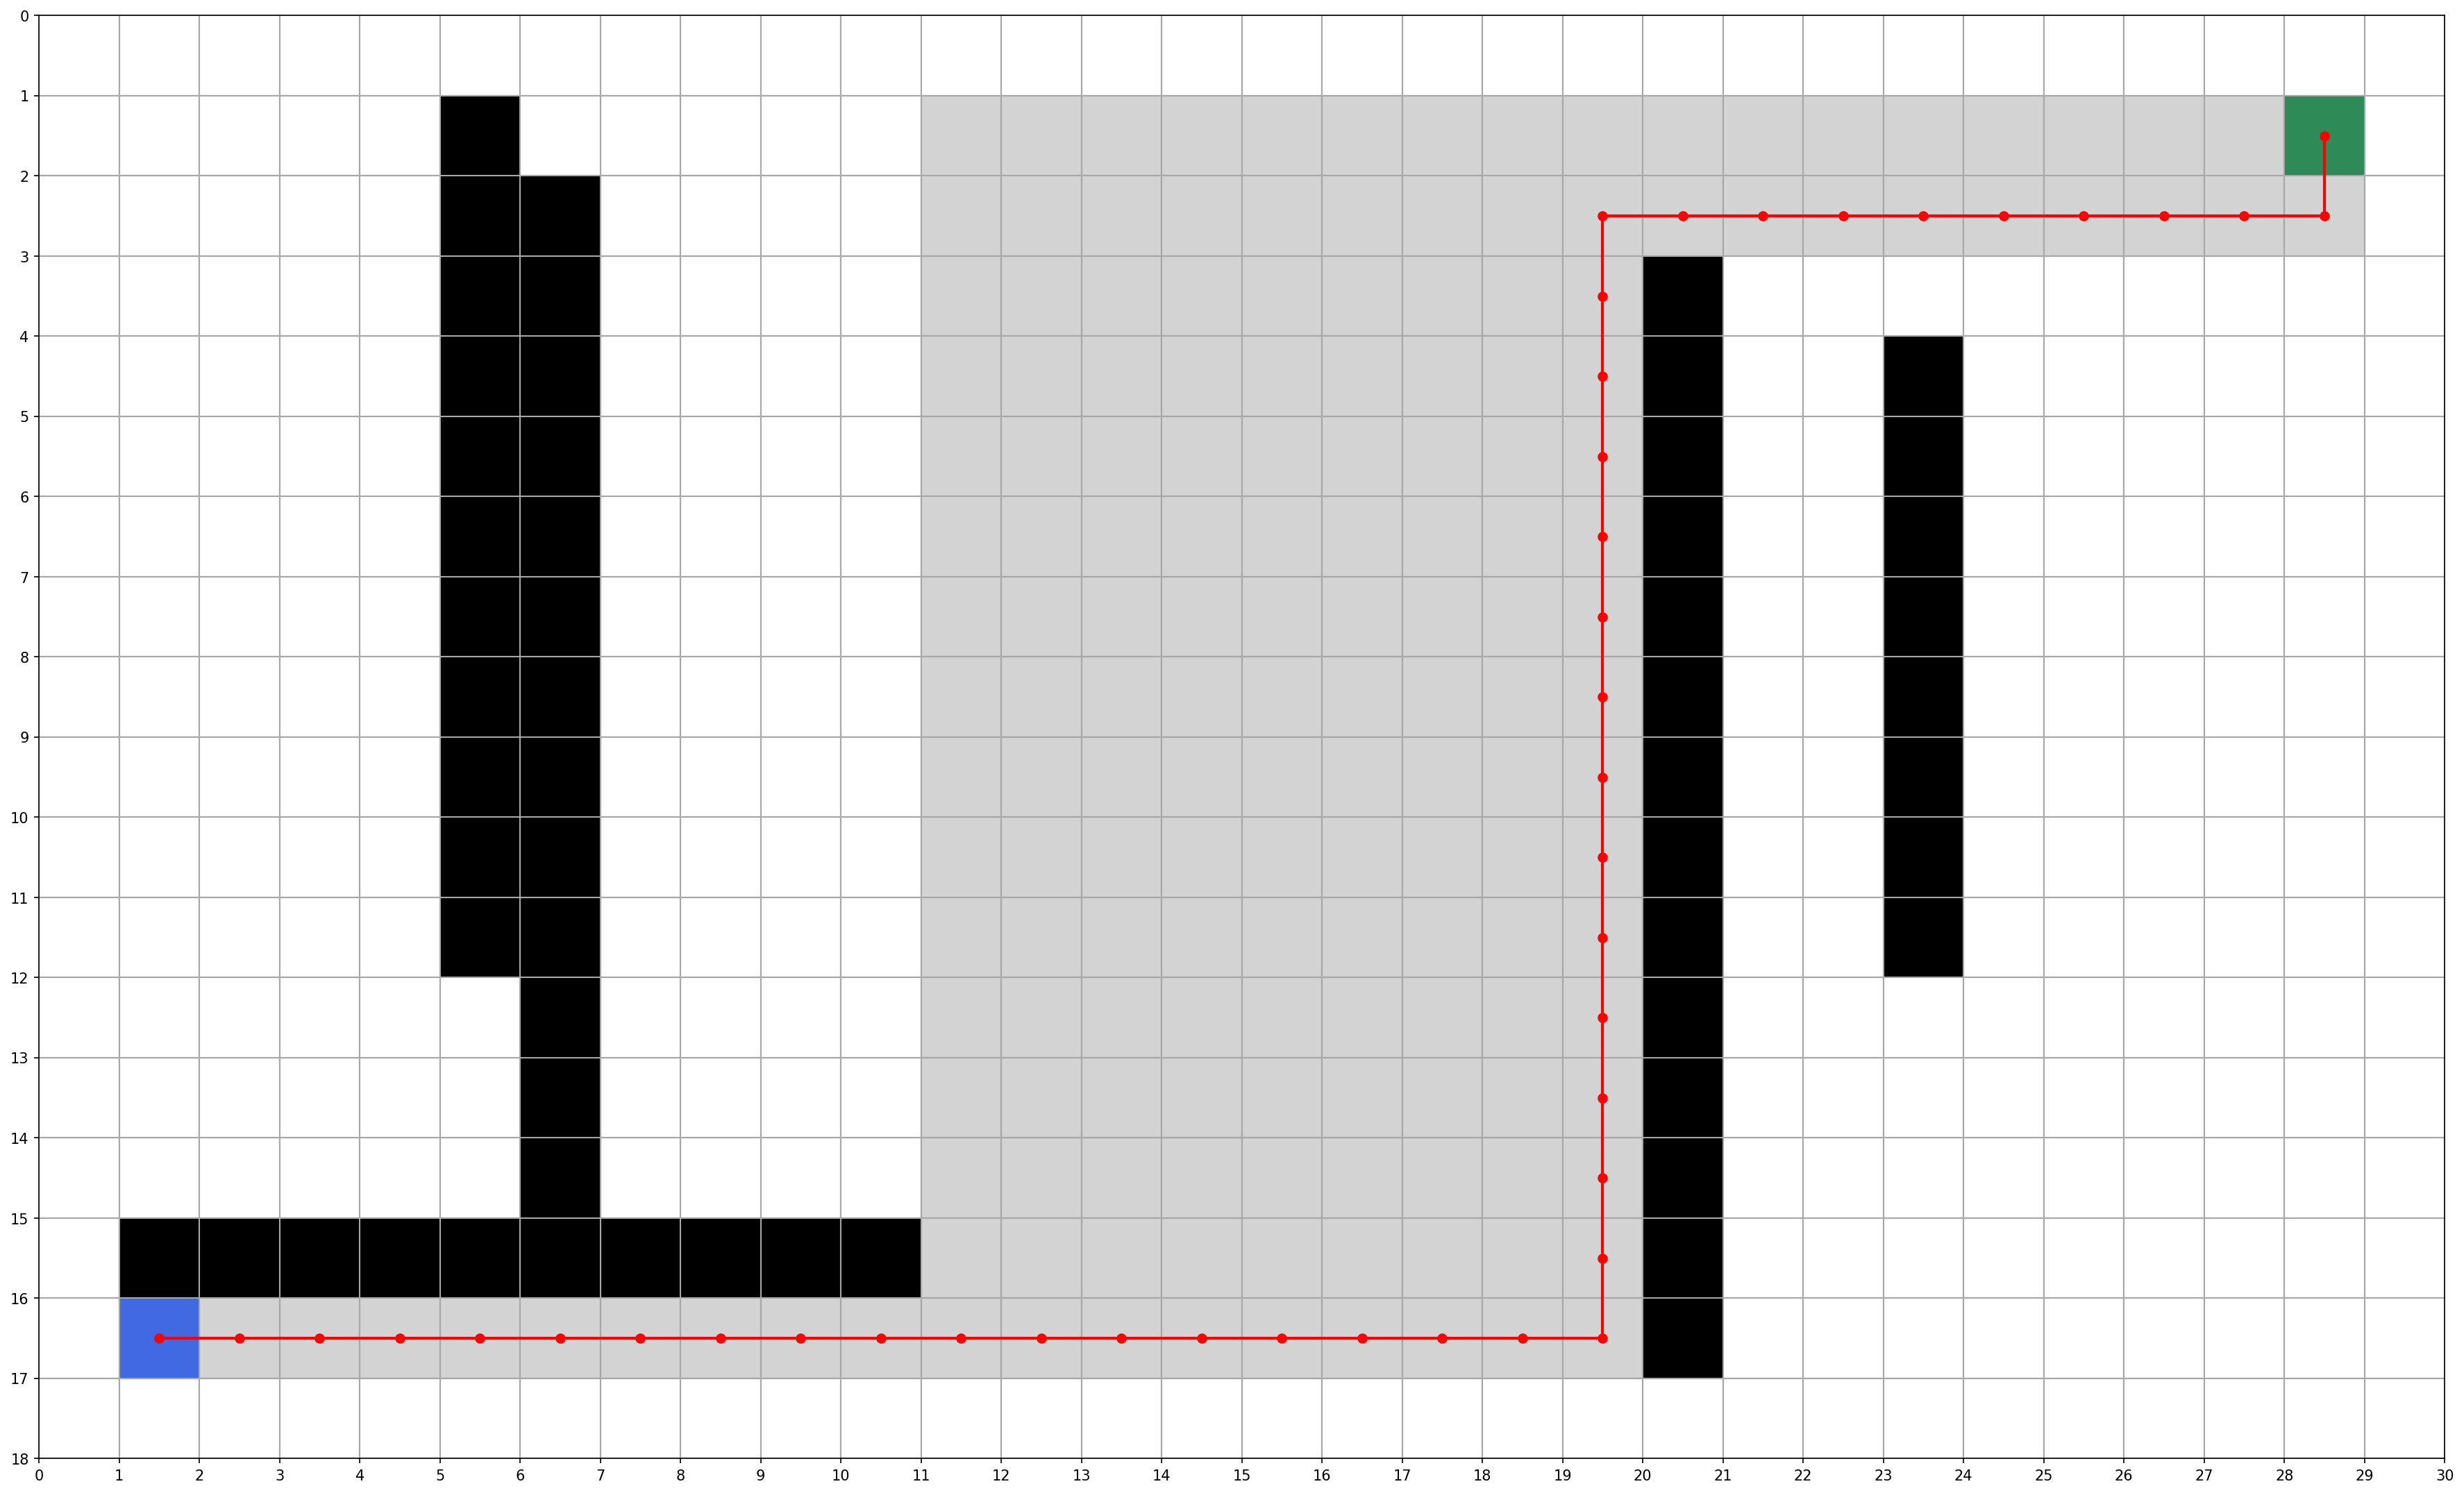
\includegraphics[width=\textwidth]{../Resultat/Recherche_de_chemin/Experimentation/visu_niveau3_difficile_baseline_etoile.png}
\end{minipage}
\hfill
\begin{minipage}{0.48\textwidth}
\centering
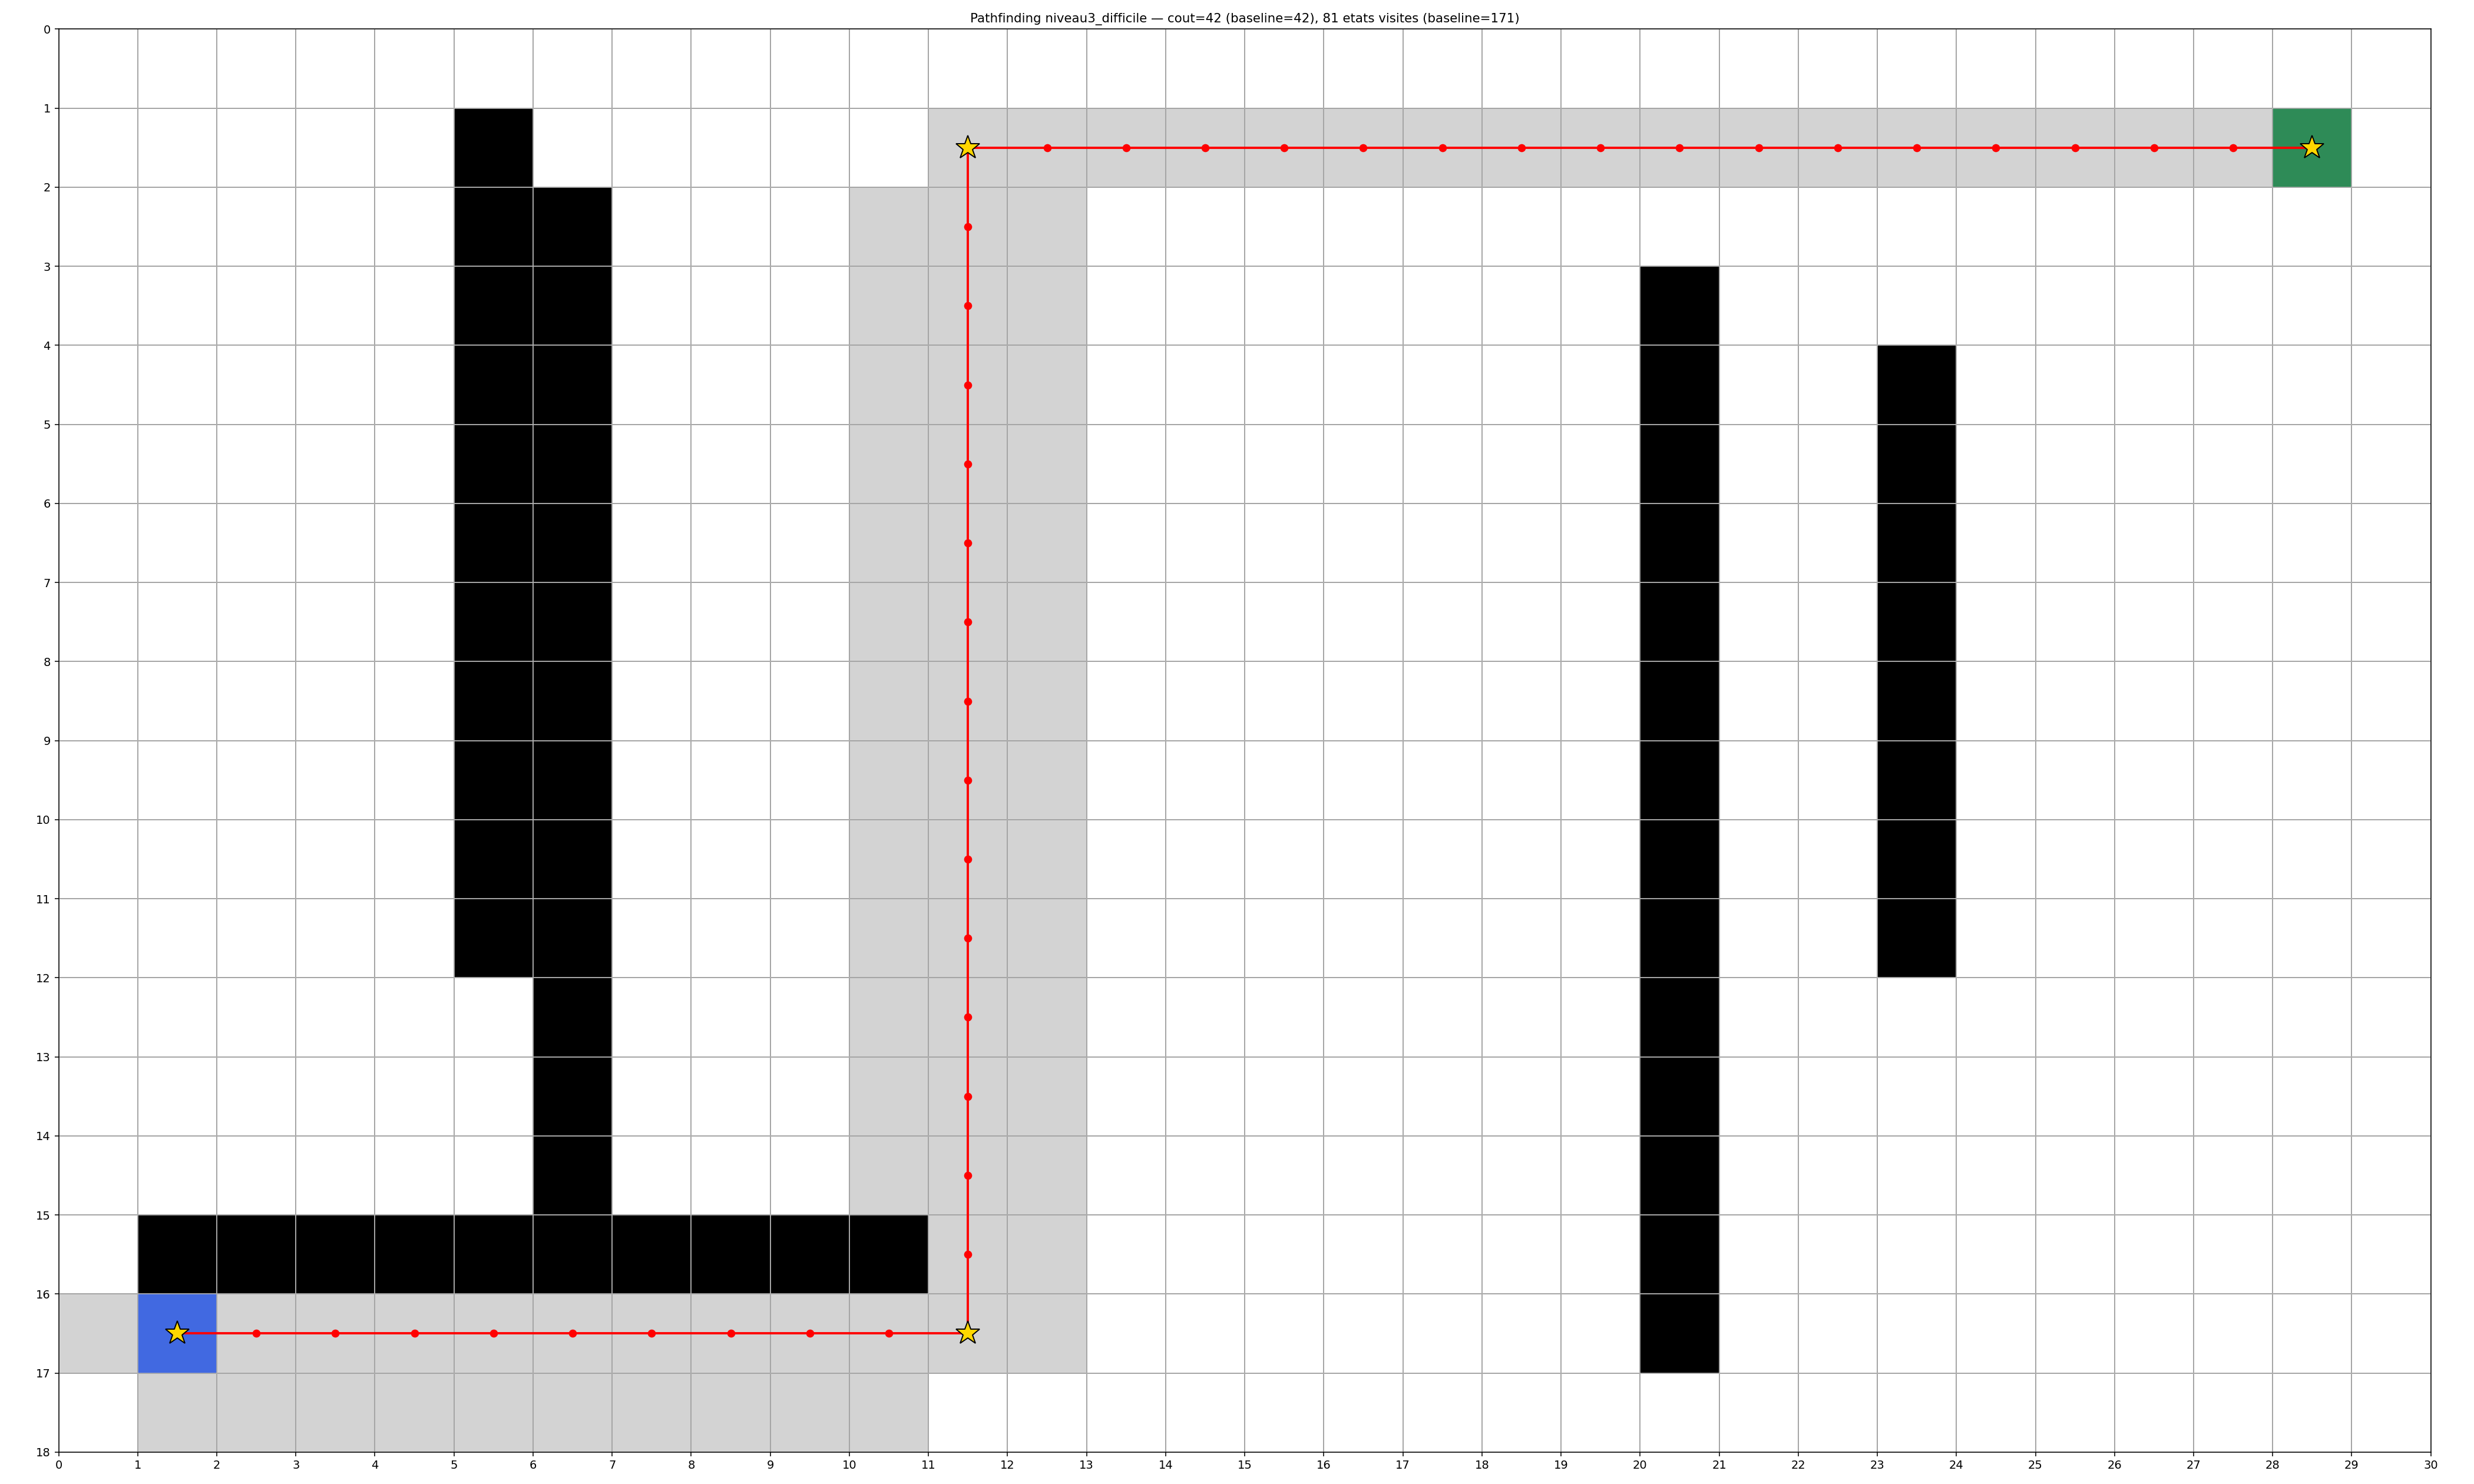
\includegraphics[width=\textwidth]{../Resultat/Recherche_de_chemin/Experimentation/visu_niveau3_difficile_waypoints_etoile.png}
\end{minipage}
\caption{Recherche de chemin niveau3\_difficile. À gauche, A* (171
états visités). À droite, LLM-A* avec Claude (81 états visités), à
coût identique, avec 2 points de passage intermédiaires repérant
le couloir libre du labyrinthe.}
\end{figure}

Les points 1 et 2 gagnent peu, quelques états en moins sur niveau1 et
niveau2, un effet nul sur niveau3 une fois le budget de 150 appels
épuisé. LLM-A* gagne beaucoup plus, jusqu'à diviser par 2 à 3 le nombre
d'états visités selon l'instance, pour un seul appel API au lieu de
150.

\subsection{Résultats pour Taquin}

\begin{table}[H]
\centering
\small
\resizebox{\textwidth}{!}{%
\begin{tabular}{@{}llccl@{}}
\toprule
Instance & Variante & Coût & Visites & Appels API \\
\midrule
niveau2\_moyen & A* & 13 & 55 & 0 \\
niveau2\_moyen & point 1 (\texttt{departager\_llm}) & 13 & 54 & 49 \\
niveau2\_moyen & point 2 (\texttt{heuristique\_llm\_lot}) & 13 & 55 & 54 \\
\midrule
niveau2\_moyen & LLM-A* & 13 & 30 (Claude), 38 (DeepSeek) & 1 \\
\midrule
niveau3\_difficile & A* & 16 & 48 & 0 \\
niveau3\_difficile & point 1 (\texttt{departager\_llm}) & 16 & 48 & 36 \\
niveau3\_difficile & point 2 (\texttt{heuristique\_llm\_lot}) & 16 & 48 & 49 \\
\midrule
niveau3\_difficile & LLM-A* & \textbf{20} (Claude), 16 (DeepSeek) & 241 (Claude), 170 (DeepSeek) & 1 \\
\bottomrule
\end{tabular}%
}
\caption{Taquin, tous les mécanismes comparés (mêmes variantes que pour
Recherche de chemin). Points 1 et 2 avec DeepSeek. LLM-A* avec Claude et
DeepSeek. Sur niveau3, Claude casse l'optimalité, coût 20 au lieu de
l'optimum réel 16, et les deux fournisseurs visitent bien plus d'états
que le baseline.}
\label{tab:taquin-tout}
\end{table}

Les points 1 et 2 restent optimaux sur les deux niveaux, comme attendu
théoriquement, mais l'effet mesuré reste très faible. Sur
niveau2\_moyen, LLM-A* reste optimal et visite moins d'états, avec de
vrais points de passage. Sur niveau3\_difficile, le tableau se
retourne. Claude casse l'optimalité, reproductible sur les 3 cartes
testées (table~\ref{tab:taquin-tout} et essais complémentaires). Les
deux fournisseurs visitent en plus bien plus d'états que le baseline,
jusqu'à 5 fois plus, alors même qu'ils proposent de vraies dispositions
intermédiaires. Le raisonnement du LLM n'est donc pas seulement
insuffisant sur ce niveau, il devient contre-productif.

\subsection{Résultats pour Sokoban}
\label{sec:claude-vs-deepseek}

\begin{table}[H]
\centering
\footnotesize
\resizebox{\textwidth}{!}{%
\begin{tabular}{@{}llccl@{}}
\toprule
Instance & Variante & Coût & Visites & Appels API \\
\midrule
microban niveau0 & A* & 1 & 1 & 0 \\
microban niveau0 & point 1 (\texttt{departager\_llm}) & 1 & 1 & 0 \\
microban niveau0 & point 2 (\texttt{heuristique\_llm\_lot}) & 1 & 1 & 2 \\
microban niveau0 & point 3 (\texttt{elaguer\_llm}) & 1 & 1 & 1 \\
\midrule
microban niveau0 & LLM-A* & 1 & 1 (Claude, DeepSeek) & 1 \\
\midrule
microban niveau1 & A* & 30 & 1088 & 0 \\
microban niveau1 & point 1 (\texttt{departager\_llm}) & 30 & 1088 & 150 \\
microban niveau1 & point 2 (\texttt{heuristique\_llm\_lot}) & 30 & 1088 & 150 \\
microban niveau1 & point 3 (\texttt{elaguer\_llm}) & 30 & 1088 & 150 \\
\midrule
microban niveau1 & LLM-A* & 30 & 819 (Claude, DeepSeek) & 1 \\
\midrule
microban niveau2 & A* & 66 & 1761 & 0 \\
microban niveau2 & point 1 (\texttt{departager\_llm}) & 66 & 1761 & 150 \\
microban niveau2 & point 2 (\texttt{heuristique\_llm\_lot}) & 66 & 1761 & 150 \\
microban niveau2 & point 3 (\texttt{elaguer\_llm}) & 66 & 1761 & 150 \\
\midrule
microban niveau2 & LLM-A* & 66 & \textbf{1814} (Claude), 1626 (DeepSeek) & 1 \\
\midrule
microban niveau3 & A* & 81 & 13\,428 & 0 \\
microban niveau3 & point 1 (\texttt{departager\_llm}) & 81 & 13\,428 & 150 \\
microban niveau3 & point 2 (\texttt{heuristique\_llm\_lot}) & 81 & 13\,428 & 150 \\
microban niveau3 & point 3 (\texttt{elaguer\_llm}) & 81 & 13\,428 & 150 \\
\midrule
microban niveau3 & LLM-A* & 81 & 11\,671 (Claude), \textbf{13\,540} (DeepSeek) & 1 \\
\midrule
microban niveau4 & A* & 89 & 56\,240 & 0 \\
microban niveau4 & point 1 (\texttt{departager\_llm}) & 89 & 56\,240 & 150 \\
microban niveau4 & point 2 (\texttt{heuristique\_llm\_lot}) & 89 & 56\,240 & 150 \\
microban niveau4 & point 3 (\texttt{elaguer\_llm}) & 89 & 56\,240 & 150 \\
\midrule
microban niveau4 & LLM-A* & 89 & 51\,065 (Claude), 50\,924 (DeepSeek) & 1 \\
\midrule
original niveau1 & A* & échec & 250\,000 (plafond) & 0 \\
original niveau1 & point 1 (\texttt{departager\_llm}) & \emph{non mesurable} & \emph{--} & \emph{--} \\
original niveau1 & point 2 (\texttt{heuristique\_llm\_lot}) & \emph{non tenté} & \emph{--} & \emph{--} \\
original niveau1 & point 3 (\texttt{elaguer\_llm}) & \emph{non tenté} & \emph{--} & \emph{--} \\
\midrule
original niveau1 & LLM-A* & \emph{non mesurable} & 250\,000 (plafond) & 1 \\
\bottomrule
\end{tabular}%
}
\caption{Sokoban, tous les mécanismes comparés. Points 1, 2 et 3 avec
DeepSeek. LLM-A* avec Claude et DeepSeek. Sur niveau2 et niveau3, un des
deux fournisseurs visite plus d'états que le baseline, en gras.}
\label{tab:sokoban-officiel}
\end{table}

Les points 1, 2 et 3 n'ont ici strictement aucun effet mesurable, sur
aucun niveau microban. Le budget de 150 appels API est négligeable face
à des espaces de 1\,000 à 56\,000 états et plus, si bien que le LLM
n'influence qu'une poignée de décisions précoces, jamais suffisant pour
changer une seule décision mesurable. LLM-A*, à l'inverse, ne casse
jamais l'optimalité ici, même avec de vraies dispositions
intermédiaires. Le nombre d'états visités baisse sur la plupart des
niveaux, mais pas partout. Sur niveau2 avec Claude et niveau3 avec
DeepSeek, LLM-A* visite plus d'états que le baseline, malgré un vrai
raisonnement à chaque fois. Sur original niveau1, le seul appel de
LLM-A* ne suffit de toute façon pas à éviter le mur des 250\,000 états,
comme la baseline.

\subsection{Réponse à la problématique}

Revenons à la question de recherche posée en introduction. Peut-on
insérer un LLM à des points précis d'un algorithme A* sans casser
l'optimalité, et à quel prix réel, en appels API et en gain mesuré ?

Pour les points 1 et 2, l'optimalité reste garantie. Le prix payé est
élevé, jusqu'à 150 appels API par instance, pour un gain mesuré nul.
Ils ne fonctionnent tout simplement pas, une fois bornés par un budget
d'appels réaliste. Les garanties théoriques posées dessus semblent
finalement plus brider le LLM qu'autre chose.

LLM-A*, à l'inverse, exploite la pleine puissance du LLM, précisément
parce qu'il ne le bride pas. Il ne coûte qu'un seul appel API par
instance. Sur Recherche de chemin, il réduit presque toujours le nombre
d'états visités, à coût optimal. Sur Sokoban, le coût reste toujours
optimal, mais le nombre d'états visités ne baisse pas systématiquement.
Sur Taquin niveau3\_difficile, le risque se matérialise vraiment.
L'optimalité casse parfois, et le nombre d'états visités augmente le
plus souvent, jusqu'à 5 fois plus qu'un A* classique, même avec un vrai
raisonnement du LLM.

Le jeu compte aussi beaucoup, tout comme la façon dont on décrit son
état. Le nombre de combinaisons possibles joue également. Sur Recherche
de chemin, l'espace de coordonnées reste simple, et LLM-A* y est
presque toujours utile. Sur Taquin et Sokoban, l'espace de dispositions
complètes est bien plus grand, et le gain devient inconstant, parfois
même négatif.

Généraliser ce mécanisme à tous les problèmes reste donc compliqué.
Sokoban original niveau1 se heurte au même mur de 250\,000 états que la
baseline classique, même avec LLM-A*, précisément le jeu le plus
difficile de nos trois. Taquin niveau3\_difficile montre en plus qu'un
vrai raisonnement du LLM ne suffit pas toujours à aider la recherche,
et peut même la ralentir.

% ============================================================
\begin{thebibliography}{9}

\bibitem{meng2024llmastar}
Meng, S., Wang, Y., et al. (2024).
\emph{LLM-A*: Large Language Model Enhanced Incremental Heuristic Search on Path Planning}.
\href{https://arxiv.org/abs/2407.02511}{arXiv:2407.02511}.

\end{thebibliography}

\begin{comment}
\subsection{Autres résultats}
\label{sec:resultats-waypoints}

\subsubsection*{Position du joueur, où plus de contexte donne moins de fiabilité}

Pour Sokoban, nous avons testé une variante où le LLM précise aussi la
\textbf{position du joueur} à chaque disposition intermédiaire, et pas seulement
les caisses, ce qui est plus fidèle à la vraie difficulté du jeu puisqu'il
faut être du bon côté d'une caisse pour la pousser. Nous avons testé
cette variante sur \texttt{petit.txt}, avec Claude, à raison de 3 essais
chacun.

\begin{table}[H]
\centering
\begin{tabular}{@{}lcc@{}}
\toprule
Variante & Optimal & Coûts observés \\
\midrule
Sans position du joueur & 3/3 & 8, 8, 8 \\
Avec position du joueur & 1/3 & 9, 9, 8 \\
\bottomrule
\end{tabular}
\caption{Ajouter une contrainte supposée plus réaliste (position du
joueur) dégrade la fiabilité au lieu de l'améliorer.}
\end{table}

Ce résultat est contre-intuitif, car la version avec joueur est pourtant
plus fidèle à la mécanique réelle du jeu. L'explication la plus probable
est que le prompt devient mécaniquement plus complexe, avec deux
informations à produire par disposition au lieu d'une, ce qui multiplie
les occasions d'erreur du LLM sans que le gain de fidélité ne compense.

\subsubsection*{Représentation ASCII vs tableau}

Nous avons aussi comparé rapidement deux représentations textuelles de
l'état Sokoban transmises au LLM, une \textbf{représentation ASCII} en grille de
caractères et une \textbf{représentation tableau} en liste de listes Python, avec une
indexation explicite \texttt{tableau[y][x]}. Le test rapide n'ayant
révélé aucun avantage à la représentation tableau, la représentation
ASCII a été retenue directement comme représentation par défaut pour tous
les tests ultérieurs de ce rapport.

% ============================================================
\section{Discussion}
\label{sec:discussion}
% ============================================================

\subsection{Sûreté théorique et utilité pratique}

Les points 1 et 2, bien que rendus théoriquement sûrs moyennant les
protections décrites (section~\ref{sec:points}), n'apportent qu'un gain
modeste, voire nul, une fois un budget d'appels API réaliste imposé
(table~\ref{tab:sokoban-officiel} et résultats pour Recherche de chemin
et Taquin). La sûreté a ainsi un coût en opportunités d'action du LLM,
car le point 1 n'agit que sur de vraies égalités de $f$, qui restent
rares sur des niveaux à heuristique discriminante, et les deux points
partagent la même contrainte de budget qui s'épuise bien avant de
couvrir l'intégralité d'un espace de recherche réaliste.

\subsection{Le mécanisme du papier original, un risque démontré et pas seulement supposé}

À l'inverse, le mécanisme de dispositions qui reproduit le papier LLM-A*
n'offre aucune garantie, et nous en avons démontré concrètement les
conséquences, avec une dégradation systématique et reproductible de la
qualité de la solution sur Taquin niveau3\_difficile, sur 6 essais sur 6
et 2 fournisseurs. C'est la différence essentielle entre notre approche
et celle du papier. Là où nous pouvons prouver qu'un point d'insertion ne
peut pas casser l'optimalité, ou identifier précisément les protections
nécessaires pour l'assurer, le mécanisme original ne peut offrir cette
garantie par construction, et le risque théorique qu'il laisse ouvert se
matérialise donc effectivement, pas seulement en théorie.

\subsection{Plus de contexte n'implique pas plus de fiabilité}

Le test de la position du joueur sur Sokoban illustre un piège. Ajouter
une information objectivement pertinente au problème, à savoir où doit
être le joueur, a dégradé la fiabilité, passant de 3/3 à 1/3 optimal, au
lieu de l'améliorer, probablement parce que la complexité accrue du
prompt multiplie les occasions d'erreur plus vite qu'elle n'apporte de
précision utile.

\subsection{Mise en regard de la littérature}

Trois papiers récents corroborent indépendamment plusieurs de nos
constats. \textbf{SokoBench} \cite{sokobench2026} rapporte des
catégories d'échec, comme les « deadlock failures » et les « spatial
reasoning mistakes », qui correspondent exactement à nos propres
observations, notamment le \emph{freeze deadlock} raté par
\texttt{elaguer\_llm} (section~\ref{sec:point3}). \textbf{A Training Data
Recipe to Accelerate A* Search with Language Models}
\cite{trainingrecipe2024} attaque le même problème, celui d'un LLM comme
heuristique pour A*, mais par \emph{fine-tuning} plutôt que par
prompting, ce qui offre un point de discussion fine-tuning contre
prompting pertinent pour situer notre approche. \textbf{GVGAI-LLM}
\cite{gvgaillm2025} teste 9 LLM sur Sokoban en zero-shot direct et
conclut que les modèles de raisonnement surclassent nettement les
modèles standards, ce qui est confirmé indépendamment par nos propres
observations sur le budget de tokens consommé par le raisonnement
interne, chez Claude comme chez DeepSeek.

Aucun de ces papiers ne teste Claude sur Sokoban, si bien que nos
résultats (section~\ref{sec:claude-vs-deepseek}) apportent une donnée que
cette littérature n'a pas encore.

\subsection{Limites méthodologiques}

Le non-déterminisme des réponses LLM impose des essais répétés, à raison
de 3 par condition au minimum, pour distinguer un effet réel d'un
artefact de hasard, et une comparaison à essai unique, comme notre
premier test ASCII contre tableau, ne permet pas de conclure avec
certitude. Le budget d'appels API, fixé à 150 pour rendre
l'expérimentation praticable sur des niveaux réalistes, borne
artificiellement l'influence mesurable du LLM sur les instances les plus
grandes, ce qui reste une limite assumée et pas une faille cachée.

% ============================================================
\section{Conclusion}
\label{sec:conclusion}
% ============================================================

Ce projet répond positivement, mais avec nuance, à sa question de
recherche. Un LLM peut bien être inséré dans A* à des points précis sans
casser l'optimalité. Le point 1, qui ordonne les nœuds, l'est par
construction, et le point 2, l'heuristique, peut l'être moyennant deux
protections indépendantes, l'admissibilité et la consistance, chacune
nécessaire mais insuffisante seule, ce que nous avons démontré par
contre-exemples exécutables et pas seulement par argument théorique. Le
point 3, l'élagage, ne peut en revanche structurellement recevoir aucune
protection sur Sokoban, un fait qui se déduit de la lecture du code,
puisque la règle classique agit déjà en amont, plutôt que d'une limite de
temps.

Le mécanisme du papier LLM-A* original, à l'inverse, n'offre aucune de
ces garanties, et nous avons montré que ce n'est pas qu'un risque
théorique, puisqu'il dégrade effectivement et de façon reproductible la
qualité de la solution sur au moins une instance testée.

La sûreté a cependant un prix. Sous un budget d'appels API réaliste,
l'apport mesuré des points protégés reste marginal, voire nul, sur la
plupart des instances traitables classiquement par A*, ce qui interroge
l'intérêt économique réel de l'approche, indépendamment de sa sûreté
théorique. Enfin, un bug de performance en $O(N^2)$ sur les plateaux
d'égalité larges a été découvert et documenté sur l'instance la plus
difficile testée, ce qui rappelle qu'une garantie de correction n'est pas
une garantie de praticabilité.

% ============================================================
\appendix
\section{Annexes}
% ============================================================

\subsection{Pourquoi IDA* est désavantagé sur Sokoban}

Nous mesurons le taux de redondance, c'est à dire le nombre d'appels
totaux à \texttt{chercher()} divisé par le nombre d'états distincts
explorés, sur une instance de difficulté moyenne de chaque jeu.

\begin{table}[H]
\centering
\begin{tabular}{@{}lccc@{}}
\toprule
Domaine & États distincts & Appels totaux & Redondance \\
\midrule
Recherche de chemin & 53 & 908 & 17$\times$ \\
Taquin & 43 & 119 & 2,8$\times$ \\
Sokoban & 1425 & 252\,305 & \textbf{177$\times$} \\
\bottomrule
\end{tabular}
\caption{IDA* n'a aucune mémoire globale des états déjà vus, si bien que
chaque transposition, c'est à dire deux chemins menant au même état,
refait tout le travail. Sokoban, où le joueur peut se déplacer librement
autour des caisses sans les toucher, est un cas extrême de
transpositions.}
\end{table}

\subsection{Pruning classique de Sokoban, coins et couloirs morts}

\begin{table}[H]
\centering
\begin{tabular}{@{}lccc@{}}
\toprule
Niveau & Avant (coin seul) & Après (+ couloirs) & Réduction \\
\midrule
niveau1\_facile & 1438 & 1088 & $-24\%$ \\
niveau2\_moyen & 9908 & 1761 & $\mathbf{-82\%}$ \\
niveau3\_difficile & 32\,287 & 13\,428 & $-58\%$ \\
niveau4\_tres\_difficile & 144\,749 & 56\,240 & $-61\%$ \\
\bottomrule
\end{tabular}
\caption{Ajouter la règle des couloirs morts, qui généralise le coin à
toute une ligne sans cible, réduit fortement l'espace exploré, sans
changer le coût optimal sur aucun niveau, ce qui montre l'absence de
faux positif.}
\end{table}

Sur le vrai niveau 1 original, publié par Thinking Rabbit en 1988 avec 6
caisses, même avec ces deux règles et 23 cases mortes détectées, la
recherche n'aboutit toujours pas après 3 millions d'états explorés
en 111s, ce qui est cohérent avec la réputation du jeu, souvent qualifié
de « Go des puzzles ». C'est pourquoi nous utilisons Microban, de
Skinner, comme corpus principal, puisqu'il reprend les mêmes vraies
mécaniques Sokoban tout en restant abordable.

\subsection{Protections activables et désactivables}

Les deux protections du point 2, \texttt{proteger\_consistance} dans
\texttt{a\_etoile()} et \texttt{proteger\_admissibilite} dans
\texttt{heuristique\_llm\_lot()}, restent désactivables pour observer le
comportement brut du LLM. Nous les testons sur
\texttt{niveau1\_facile/carte1}, pour Recherche de chemin.

\begin{table}[H]
\centering
\begin{tabular}{@{}lccc@{}}
\toprule
Variante & Coût & Visites \\
\midrule
Aucune protection & 10 & 28 \\
Consistance seule (pathmax) & 10 & 30 \\
Admissibilité seule (min) & 10 & 33 \\
Les deux protections & 10 & 33 \\
\bottomrule
\end{tabular}
\caption{Sur cette instance précise, le coût reste optimal dans les 4
cas, car l'heuristique classique du jeu, déjà consistante, limite le
risque observable ici. Les contre-exemples construits à la main
(section~\ref{sec:point2}) restent donc nécessaires pour démontrer le
risque en général.}
\end{table}

\iffalse
% Preuve commentée pour l'instant, on y reflechit encore -- gardee au cas
% ou on voudrait la remettre plus tard.
\subsection{Preuve d'optimalité de A*, heuristique consistante et recherche par graphe}
\label{sec:preuve-optimalite}

Cette démonstration complète est écrite pour correspondre exactement à
notre implémentation, qui fait une recherche par graphe où un état fermé
n'est jamais rouvert, et pas la version « manuel » habituelle, avec une
recherche par arbre et l'admissibilité seule. C'est cette preuve, et
précisément l'endroit où elle exige la consistance, que le contre-exemple
de la section~\ref{sec:point2} casse concrètement.

\paragraph{Cadre.} On considère un graphe d'états dont les arêtes ont un
coût strictement positif, et on note $g^*(n)$ le coût réel du plus court
chemin départ~$\to$~$n$. $h$ est dite consistante si, pour toute arête
$(n \to n')$ de coût $c(n,n')$,
\[
h(n) \le c(n,n') + h(n'), \qquad h(\text{but}) = 0 \text{ pour tout état but.}
\]
A* dépile toujours le $f = g+h$ minimal de \texttt{ouverts}, et ne rouvre
jamais un état une fois dans \texttt{fermes}.

\paragraph{Théorème.} Si $h$ est consistante, alors quand A* dépile un
état but et s'arrête, $g(\text{but}) = g^*(\text{but})$, et aucune
solution moins chère n'existe ailleurs dans le graphe.

\paragraph{Lemme 1 (monotonicité de $f$ le long d'un chemin).} Le long de
n'importe quel chemin $n_0 \to n_1 \to \dots \to n_k$ (coûts réels
cumulés $g^*(n_i)$), la quantité $f^*(n_i) := g^*(n_i) + h(n_i)$ est
non-décroissante.

\emph{Preuve.} Pour deux nœuds consécutifs, on a
\begin{align*}
f^*(n_{i+1}) &= g^*(n_{i+1}) + h(n_{i+1}) \\
             &= g^*(n_i) + c(n_i,n_{i+1}) + h(n_{i+1}) \\
             &\ge g^*(n_i) + h(n_i)
             \qquad \text{(par consistance, } h(n_i) \le c(n_i,n_{i+1}) + h(n_{i+1}) \text{)} \\
             &= f^*(n_i).
\end{align*}
Par récurrence, $f^*$ est non-décroissante sur tout le chemin. $\blacksquare$

\paragraph{Lemme 2, l'invariant clé selon lequel un état fermé a toujours le bon $g$.}
Quand A* ferme un état $n$, $g(n) = g^*(n)$.

\emph{Preuve (par l'absurde).} D'abord, $g(n)$ ne peut jamais être
strictement inférieur à $g^*(n)$, car $g(n)$ est toujours le coût d'un
vrai chemin trouvé, et $g^*$ est le minimum sur tous les chemins. La seule
erreur possible serait donc $g(n) > g^*(n)$.

Supposons que ce soit le cas, et soit $n$ le premier état fermé par A*
avec $g(n) > g^*(n)$, de sorte que tout état fermé avant lui a un $g$
correct.

Considérons le vrai plus court chemin départ~$\to$~$n$, de coût
$g^*(n) < g(n)$. Le départ est fermé dès le début avec un $g$ correct
($g(\text{départ}) = 0 = g^*(\text{départ})$), et $n$ lui-même n'est pas
encore fermé au moment où on le ferme. Il existe donc, le long de ce
chemin, un dernier état $p$ déjà fermé, avec un $g$ correct par
minimalité de $n$, suivi d'un état $p'$, successeur de $p$ sur ce même
chemin, qui n'est pas encore fermé à cet instant.

Comme $p$ a été fermé, tous ses voisins (dont $p'$) ont déjà été générés
et poussés dans \texttt{ouverts}, avec un $g$ au plus égal à
$g(p) + c(p,p') = g^*(p) + c(p,p') = g^*(p')$ (puisque $p'$ est sur le
plus court chemin vers $n$ via $p$). Et comme $g$ ne peut jamais être
strictement en dessous de $g^*$, on a donc exactement
\[
g(p') = g^*(p') \qquad \text{donc} \qquad f(p') = g^*(p') + h(p') = f^*(p').
\]
Or $p'$ est sur le plus court chemin départ~$\to$~$n$, donc par le
Lemme~1 appliqué au tronçon restant $p' \to \dots \to n$, on obtient
\[
f^*(p') \le f^*(n) = g^*(n) + h(n).
\]
Et comme $g(n) > g^*(n)$ par hypothèse, on a alors
\[
f(p') = f^*(p') \le g^*(n) + h(n) < g(n) + h(n) = f(n).
\]
Donc $f(p') < f(n)$, avec $p'$ toujours dans \texttt{ouverts} à l'instant
où A* choisit de dépiler $n$. Mais A* dépile toujours le $f$ minimal de
\texttt{ouverts}, ce qui est une contradiction, puisque $p'$ était
disponible avec un $f$ strictement plus petit.

Donc aucun tel $n$ n'existe, et tout état fermé a toujours
$g(n) = g^*(n)$. $\blacksquare$

\paragraph{Conclusion du théorème.} Soit \emph{but} l'état que A* dépile
et ferme le premier parmi les états satisfaisant le test de but. Par le
Lemme~2, $g(\text{but}) = g^*(\text{but})$, et comme $h(\text{but}) = 0$,
$f(\text{but}) = g(\text{but}) = g^*(\text{but})$.

Reste à écarter l'existence d'une solution moins chère ailleurs.
Supposons qu'il existe un chemin départ~$\to$~$\text{but}_2$ (un autre
état but, ou même le même) de coût réel $C^* < g(\text{but})$. Par le
même argument de frontière que dans le Lemme~2, avec un dernier nœud déjà
fermé sur ce chemin alternatif, suivi d'un nœud $q$ pas encore fermé, avec
$g(q) = g^*(q)$ exact, et par le Lemme~1 appliqué au tronçon
$q \to \dots \to \text{but}_2$, on obtient
\[
f(q) = f^*(q) \le f^*(\text{but}_2) = g^*(\text{but}_2) + h(\text{but}_2) = C^* + 0 = C^*.
\]
$q$ est dans \texttt{ouverts} au moment où A* dépile \emph{but}. Comme A*
a choisi \emph{but} plutôt que $q$, on a alors
\[
f(\text{but}) \le f(q) \le C^*.
\]
Donc $g^*(\text{but}) = f(\text{but}) \le C^*$, ce qui contredit
$C^* < g(\text{but}) = g^*(\text{but})$. Aucune solution moins chère
n'existe. $\blacksquare$

\medskip
La preuve entière tient sur $g(p') = g^*(p')$ pour tout état fermé avant
$n$, établi au Lemme~2. Dès qu'une seule fermeture est incorrecte, avec
une heuristique admissible mais pas consistante, toute la chaîne
d'inductions s'effondre, et c'est exactement ce que reproduit le
contre-exemple exécutable de la section~\ref{sec:point2}, avec un coût
de 5 au lieu de 4.
\fi

\subsection{Ressources}

Le code source complet se trouve dans le dépôt du projet, dans les
dossiers \texttt{Algorithmes/}, \texttt{Jeux/} et \texttt{Resultat/}.
L'ensemble des prompts utilisés est documenté dans
\texttt{Resultat/prompts\_utilises.md}, et les données brutes de toutes
les expérimentations, au format CSV et JSON, sont conservées dans les
dossiers \texttt{Resultat/*/Experimentation/} et
\texttt{Resultat/Visualisation\_Waypoints/}.

\end{comment}

\end{document}
